\documentclass[letterpaper, 11pt]{Proposal}
\title{\vspace{-0.5cm}\hspace{-1.5cm}Triply} % maybe together with the platform logo
\author{Azhel Uladzislau, Bortolotti Samuele, Petrosyan Vahan, \\Sassetti Gianluca, Stolin Marcel}
\date{26th November 2021}

\def\Sec#1{Section~\ref{#1}}

\begin{document}

\vspace{-10cm}

\begin{textblock}{10}(3,1)
\textit{University of Trento}\\
\textit{Department of Computer Science}\\
\textit{Innovation and Business in ICT}
\end{textblock}

\maketitle

\begin{tikzpicture}[overlay, remember picture]
  \node[xshift=-6cm,yshift=-1.6cm] at (current page.north east) {
\includegraphics[width=4.5cm,height=1.5cm]{logo_unitn}};
\end{tikzpicture}

\begin{tikzpicture}[overlay, remember picture]
  \node[xshift=-9.9cm,yshift=-3.6cm] at (current page.north east) {
\includegraphics[width=1cm,height=1cm]{logo}};
\end{tikzpicture}

\vspace{-2cm}

\section{Platform idea}\label{sec:platform-idea}
Triply is a platform which provides information regarding points of interest nearby the users, such as sights, restaurants and entertainment centres.
The application graphical user interface is thought to be as clear and straightforward as possible, in order to be easily accessible by a vast variety of users; its main component is a map (see \Sec{sec:appendix_mockup} Mockup in the appendix), where users can point specific places out by adding a position tracker to the corresponding area so that others can visit them. Moreover, it is possible to add pictures and reviews of a place, providing a 1 to 5 stars rating and sharing a comment about personal experiences in order to let other users know if it is recommendable or not. Not only can users add places to the map, which are retained relevant or interesting, and the corresponding reviews, but also follow other users, in order to see the places they have recently visited along with their opinion on them. 

Besides writing reviews, users can chat with each other, so as to share their thoughts concerning places they have visited; it could be, therefore, a chance to meet and get to know other people with common interests. 

The added places are organised in some categories, so as to make it easier for users to find a suitable location for any kind of trip. Triply has a recommendation system based on artificial intelligence which, according to user preferences and to followed users' activities, suggests daily or weekly new places to visit.

In order to offer a more efficient service, we plan to arrange a partnership with a few rating companies, such as \emph{Tripadvisor}\footnote{\url{https://www.tripadvisor.com/}} and \emph{Google Maps}\footnote{\url{https://www.google.com/maps}}; this cooperation would allow us to incorporate their data in the platform, so as to enrich its content. Concerning the interaction between external companies and the platform users, the application allows the companies to sponsor their services regarding tourism, by adding the locations they own and the events, which take place there. The influencers community, which has rapidly grown in the last few years, brand and travel bloggers could, moreover, have a significantly positive effect on the advertisement of their products or services.

\section{Market and competition}\label{sec:mrkt-comp}
As for the market trend, the Internet has significantly changed the way people organise their trips, offering them a huge variety of possible sources to search on; according to Dan Wang et al., in fact, it appears that the number of destinations considered by the users in the travel planning process has considerably increased~\cite{travel_impact:2016}. Inevitably, traditional travel planning has lost interest among customers, since they can rely on a vast amount of information easily and freely accessible online.

As far as the market segment is concerned, the initial target of Triply, analysed from a demographic perspective, is people aged between 15 and 45 years. Furthermore, considering Triply's aim, the main clientele is undoubtedly composed of people, who either love to travel or simply want to discover new places to practise sport, and have familiarity with social networks.

In order to attract external innovation through competitive markets, the platform adopts a two-sided business model (see \Sec{sec:business_model_canvas} Business Model Canvas in the appendix), ensuring companies and potential innovators the possibility to communicate with users in order to advertise their services or products. Thanks to the influencer community, which interacts with the platform users, external companies can offer sponsorships to travel or brand bloggers, who can arouse interest in the activities they propose and in the products they sell. We expect to compete directly with our partners because they can advertise their services on our platform as well as in the app stores for smartphones.

Triply combines the user interaction and the possibility of writing and reading reviews in one brand-new application, as a result, the main competitors can be identified in social networks and review applications.
We have distinguished two types of competitors: direct and indirect. 

\subsection{Indirect competitors}
As far as indirect competitors are concerned, review platforms, such as \emph{Tripadvisor}, allow to rate and leave comments on restaurants, hotels, airlines or other attractions and guarantee a detailed search by categories and criteria. Unlike Triply, the main focus of these platforms is merely to find the best low-priced solution suitable for the user’s needs and does not involve any kind of advice or recommendation. Furthermore, common review applications do not allow users to chat with each other or to directly sponsor businesses or services within the platform. 

Platforms such as \emph{Google Maps} allow customers to locate places in their proximity and to provide reviews, but it lacks social interaction and communication between companies and customers.

Concerning social interaction, the main indirect competitors are social networks, in particular \emph{Instagram} and \emph{Facebook}, as they both enable users to develop a relationship with other users by sharing their experiences and chatting with them. Despite that, since these applications are mainly focused on social interaction, the possibility of reviewing places or services is not much considered.

\subsection{Direct competitors}
As for direct competitors, \emph{Yelp}\footnote{\url{https://www.yelp.it/}} is a review application, which provides a service linked to local businesses discovery. Users are able to review and add new businesses on the platform, which offers a recommendation system aimed to suggest the best ones located nearby the users.
Moreover, \emph{Yelp} includes a section dedicated to friends, which allows the communication and the mutual exchange of personal experiences with regard to specific businesses. 
As it is focused on businesses, users do not have the possibility to add, review and discover places not connected to a company.

Another direct competitor is \emph{Foursquare city guide}\footnote{\url{https://foursquare.com/cities}}, a platform which allows users to share their location with their friends. The application is focused on finding local attractions and writing reviews about them, suggesting to other users, whether it is worth going to or not. Moreover, \emph{Foursquare city guide} provides the possibility of adding any kind of place, which, therefore, does not necessarily need to be linked to a business. However, it does not include a social interaction service: users cannot follow each other, nor can they chat with other people on the platform.

\section{Users and monetisation}\label{sec:usrsAndMon}
In order to deepen the knowledge of the market segment, we studied the possible users of our platform through \emph{personas} (available in \Sec{sec:appendix_personas} in the appendix). We have therefore decided to classify our potential customers into two categories, the ordinary users and the business users, according to the purpose for which they use the platform.

\subsection{Ordinary Users}\label{subsec:usrsAndMon_users}
As far as ordinary users are concerned, they are end-users of our platform, who could enjoy the application and use it on a regular basis for personal purposes. The general profile of such users is a relatively young person aged between 15 and 45 years, confident with the use of smartphones and the Internet, who loves to explore new places, both tourist attractions and dining, shopping, and entertainment venues, either alone or with friends.

\subsection{Business Users}\label{subsec:usrsAndMon_business-users}
Concerning business users, they can either be individuals or companies, that generate income indirectly from the platform itself and/or advertise their business on the application, using it as a means of communication between the company and the users. Businesses which manage events can sell tickets or appointments directly on the platform. The general profile of such users is a highly motivated company which aspires to go digital and advertise their business mainly to a targeted audience. We have identified suitable examples of these businesses mainly in influencers and advertising companies, who can induce trends through the vast impact of the Internet, and in tour operators, small businesses, and entertainment companies.
As far as tour operators are concerned, such businesses may promote their trips by adding places and photos and asking for sponsorship with our platform; the same applies to small businesses and entertainment companies. In addition, businesses employed in events organisation, can ask to sell their tickets on our platform.

Regarding the acquisition of new customers, we plan to enhance the user base by adopting two strategies: the \emph{producer evangelism} and the \emph{piggyback}. Concerning the \emph{producer evangelism}, we aim to exploit the word of mouth by contacting some travel or brand bloggers to review our platform. Furthermore, we intend to ask the major social networks, such as \emph{Facebook} and \emph{Instagram}, and third-party websites, such as \emph{YouTube}, for advisement by exploiting the \emph{piggyback} approach in order to leverage on those platforms' users to promote our application.
As far as the maintenance of customers is concerned, we plan to keep our users by encouraging the liberty of expression and promoting social interaction through the recommendation of trendy places which are filtered so as to favour those in their proximity and which reflect better their interests.
The accomplished achievements and the general activity of a user can be shared on other platforms.
Concerning the growth of the number of customers, we plan to reward the highly active ones through badges in order to highlight the individual’s activity level and through the concession of verified reviews or verified profiles for trustworthy users.

\subsection{Economic perspective}\label{subsec:usrsAndMon_monetization}
In the analysis of the platform economic perspective, we have considered the financial and monetisation aspects, which are briefly outlined in the following sections.

\subsubsection{Financing}
In order to collect money to fund our venture, we have decided to rely on the following money sources. The first way, in which we plan to be financed, is to use our collective funds and those borrowed from our families and friends (3F). We consider getting financed by a Venture Capitalist as we believe it is the most suitable way to start our business and overcome the cash flow challenges such as the inventory, the employees and the advertisement, and the capital investments such as costs for the IT infrastructure. 

\subsubsection{Monetisation}
The business model of our venture is the two-sided platform, as mentioned in \Sec{sec:mrkt-comp}. Therefore, we plan to generate income by paid promotions, as other social networks or sites do, by subsidising one side strategy, charging only the business users who decide to employ the advertisement features of our application.
In fact, businesses can promote their activity through our application by paying a fee in order to advertise their place by putting their location in the recommendation lists of the users or general advertisements visible on the platform.
Another source of revenue is given by the possibility to sell tickets directly within the platform, in that case, we plan to keep 1\% of each ticket cost. In order to attract new business users, we have planned the time to start charging the companies by providing six months of free advertising to each organisation which joins the site.
Finally, we plan to gain attention by offering fast and reliable service, which aims at the satisfaction of both business and ordinary users by implementing filters so as to make sure that everyone finds what they are looking for.

\section{Potential network effects}\label{sec:network-effects}
According to Metcalfe's law, the application value depends strictly on the number and the type of users who use it; for this reason, we have analysed the platform potential network effects (see \Sec{sec:network_effects} Mockup in the appendix).

\subsection{Positive network effects}
As far as the positive network effects are concerned, we have predicted that a possible increment in the number of users may increase the value of the platform. The benefit we have considered is the increase in the number of places of interest, which will enhance the possibility of discovering suitable places for every user of the platform. 
For the law of large numbers, with the growth in the number of reviews, the rating of the place will converge to its exact value, which means that the recommendation system will perform more efficiently. Furthermore, it is obvious that if the number of ordinary users increases, the possibility for a business user to attract them grows, too. On the other hand, the increment in the number of business users leads necessarily to a greater possibility for an ordinary user to find a place of interest.

\subsection{Negative network effects}
Concerning negative network effects, one of the main problems we may face is the network congestion: in fact, the growth of users on the platform induces the need for a continuous improvement of our infrastructure and if it is not properly managed, the service may not work as expected.
Since the rise in the number of users would inevitably cause a bigger probability to attract people with disruptive behaviours, we have hired several moderators to admonish such users.
Finally, we have recognised that the more marketers there are, the more advertisements the platform displays and the less appealing it becomes to potential consumers.

\section{Potential limitations, threats, and possible solutions}
Obviously, Triply has some limitations and in order to overcome those obstacles, we have introduced several solutions (see \Sec{sec:swot} SWOT Analysis in the appendix).

First of all, during the launch (the phase entering the market) of the platform, there will be a lack of data about places of interest. For this reason, we will establish a relationship with our indirect competitors so as to integrate their data within our platform, namely locations and reviews.

Secondly, in order to avoid bad reviews, which would decrease the average rating of the locations, it will be necessary to implement the system, described below.
It will include an auto-notification algorithm, which will send an e-mail to the company about how to increase their popularity and ratings. Furthermore, the latest reviews will be considered with higher priority, so as to give less importance to the old ones. For the purpose of avoiding offensive and fake reviews, we will employ special algorithms, capable of removing them automatically. A group of moderators will be hired so as to give users the possibility to report bad behaviours and admonish or ban vandals. In order to ensure that the application meets the real needs of all users involved, we have decided to integrate feedback mechanisms so as to collect all their possible requests and then decide how to adapt the platform according to them.

As the company business objective is to grow as fast as possible, we have made user engagement our primary goal.
We plan to analyse the following \empty{KPI} on a regular basis (every two months) in order to assess our organisation's progress.
As a result, in order to enhance Triply's revenue, we aim to increase the number of active platform users by tracking the average number of website visitors, the average time spent on the application, the total number of posts per day, and the customer satisfaction. 

Finally, we have considered the privacy issue. During the registration stage, every user will receive a privacy notice according to the local-law regulations; this is why the application will be fully \emph{GDPR}\footnote{General Data Protection Regulation - \url{https://eur-lex.europa.eu/eli/reg/2016/679/oj}} compliant. As an additional feature, users will be able to add reviews anonymously in order to avoid privacy issues. 

\bibliographystyle{ieeetr}
\bibliography{bibliography}

\clearpage

\section*{Appendix}\label{sec:appendix}

\appendix

\pagenumbering{arabic} % resets `page` counter to 1
\renewcommand*{\thepage}{A\arabic{page}}

\section{Mockup}

\includegraphics[scale=0.43]{mockup}\label{sec:appendix_mockup}

\section{Business Model Canvas}

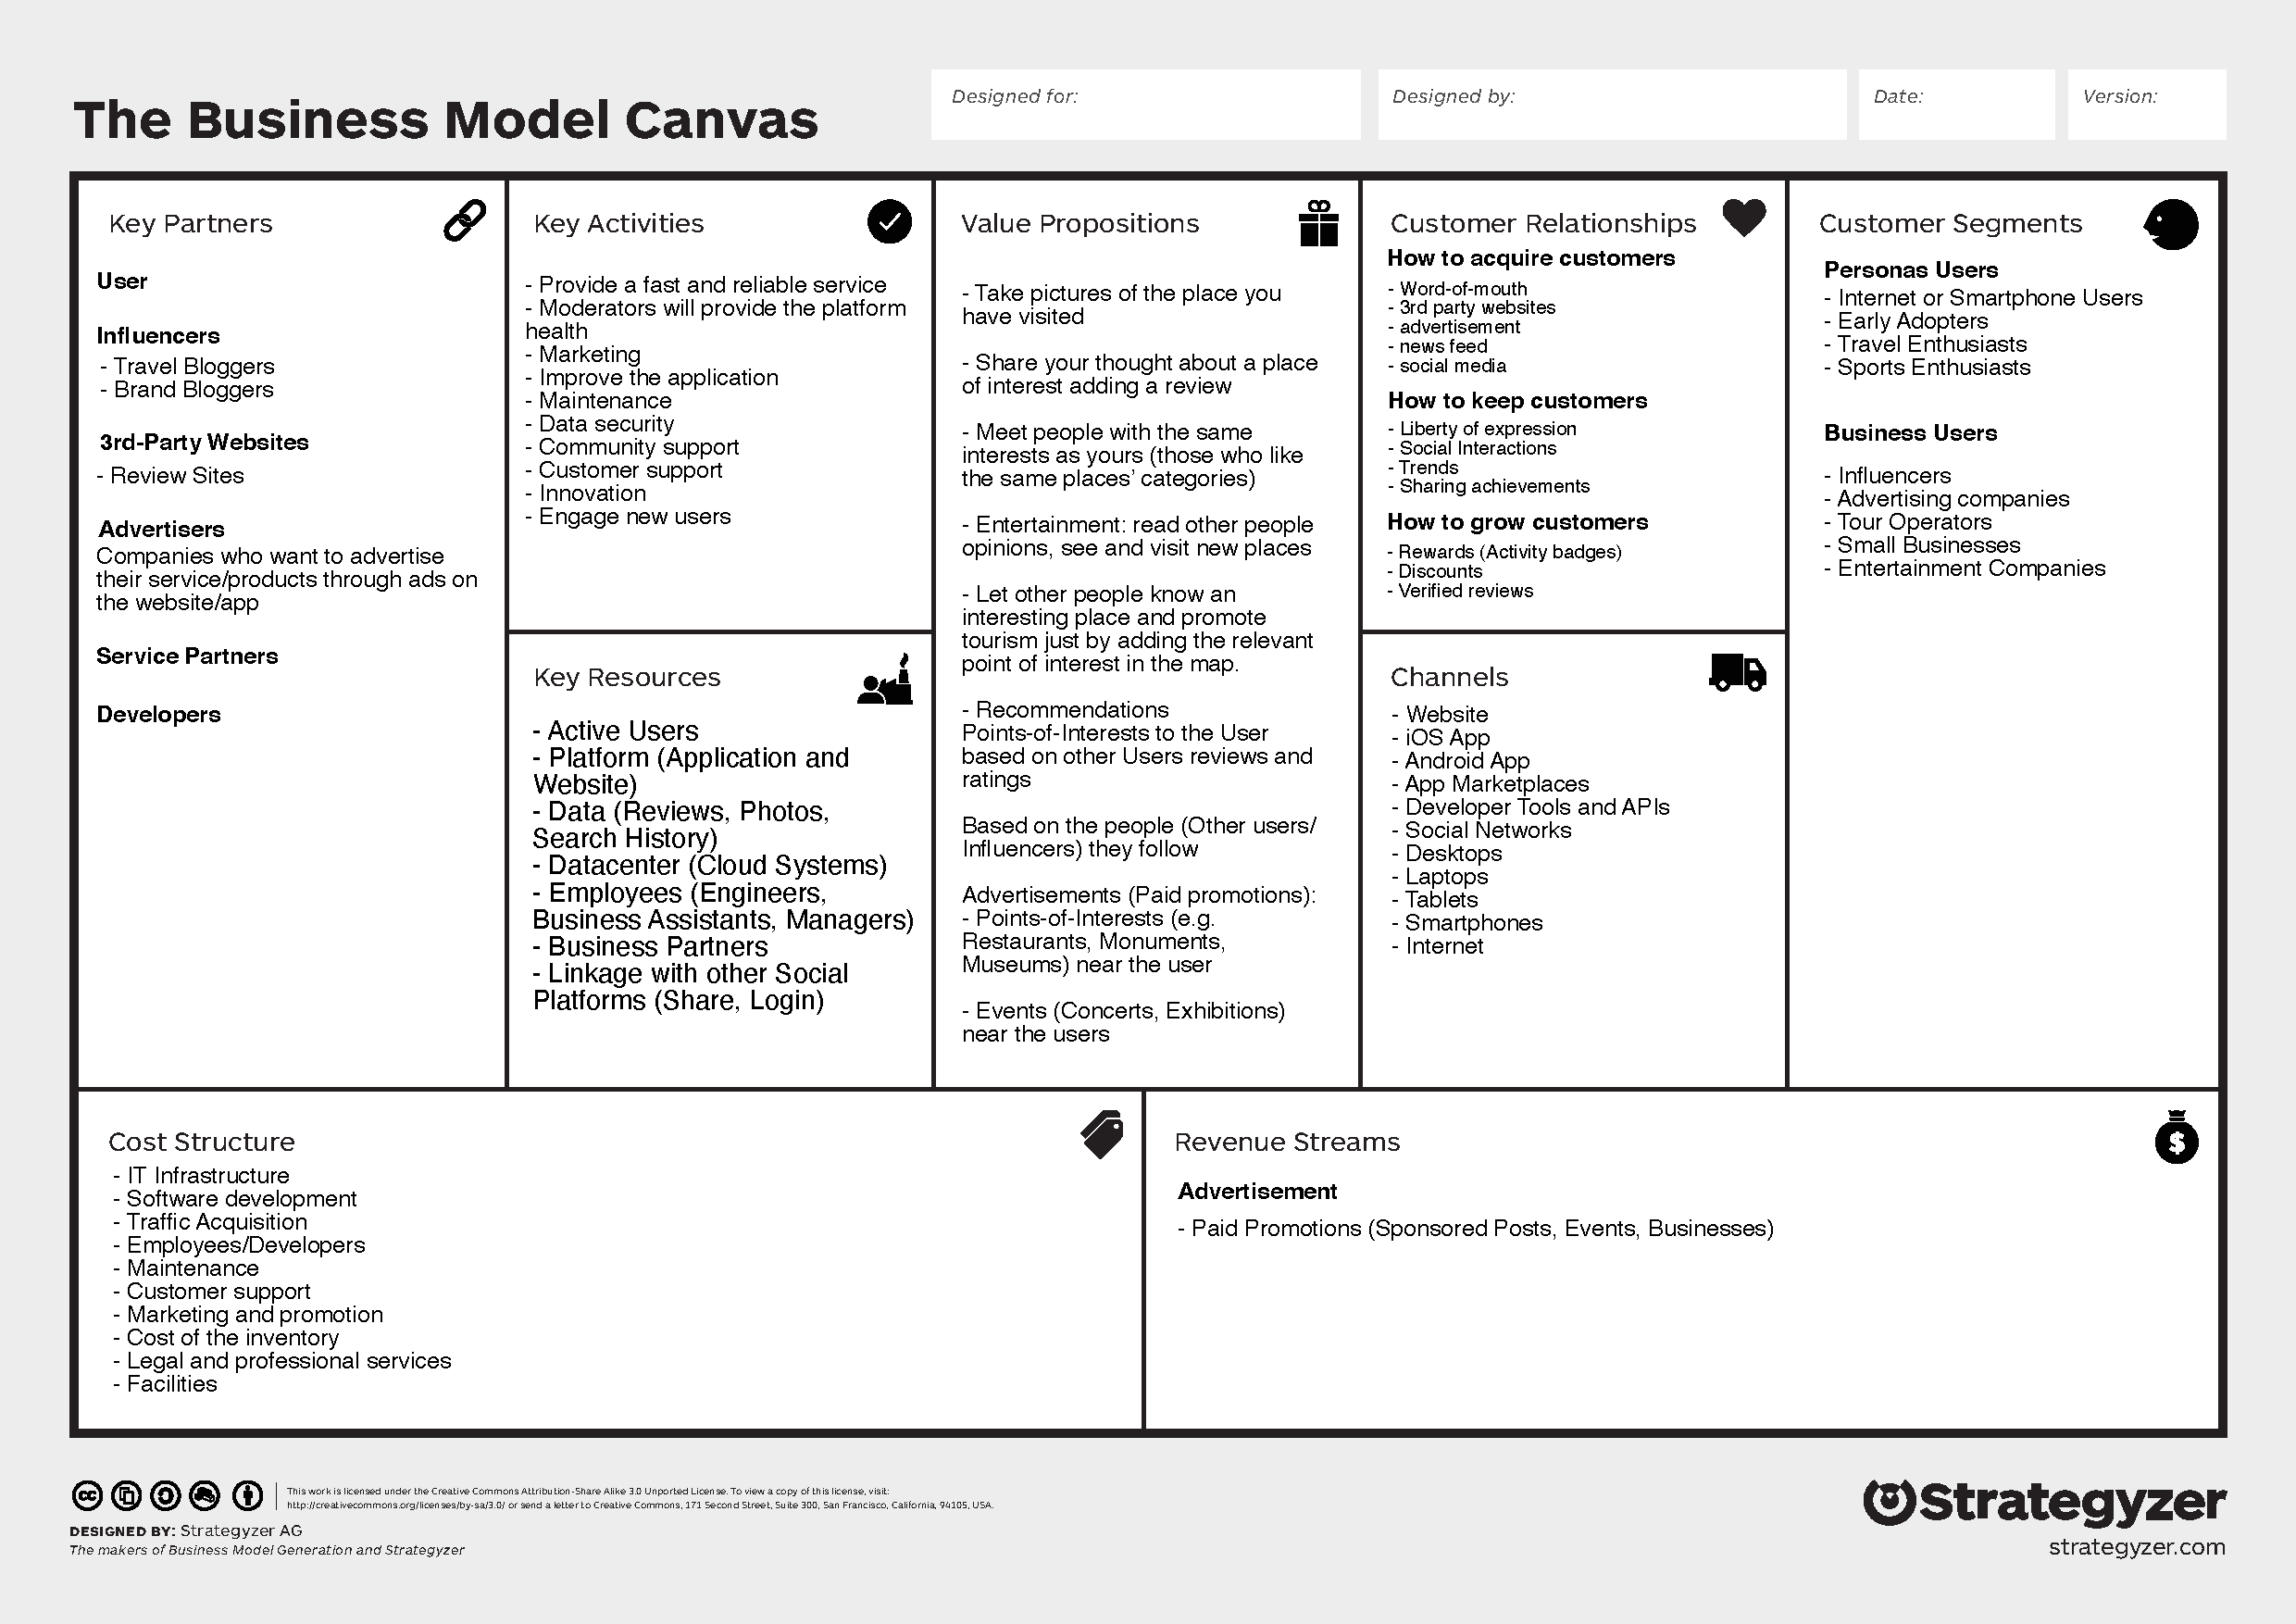
\includegraphics[scale=0.51, angle=90]{business_model_canvas}\label{sec:business_model_canvas}

\section{Personas}\label{sec:appendix_personas}

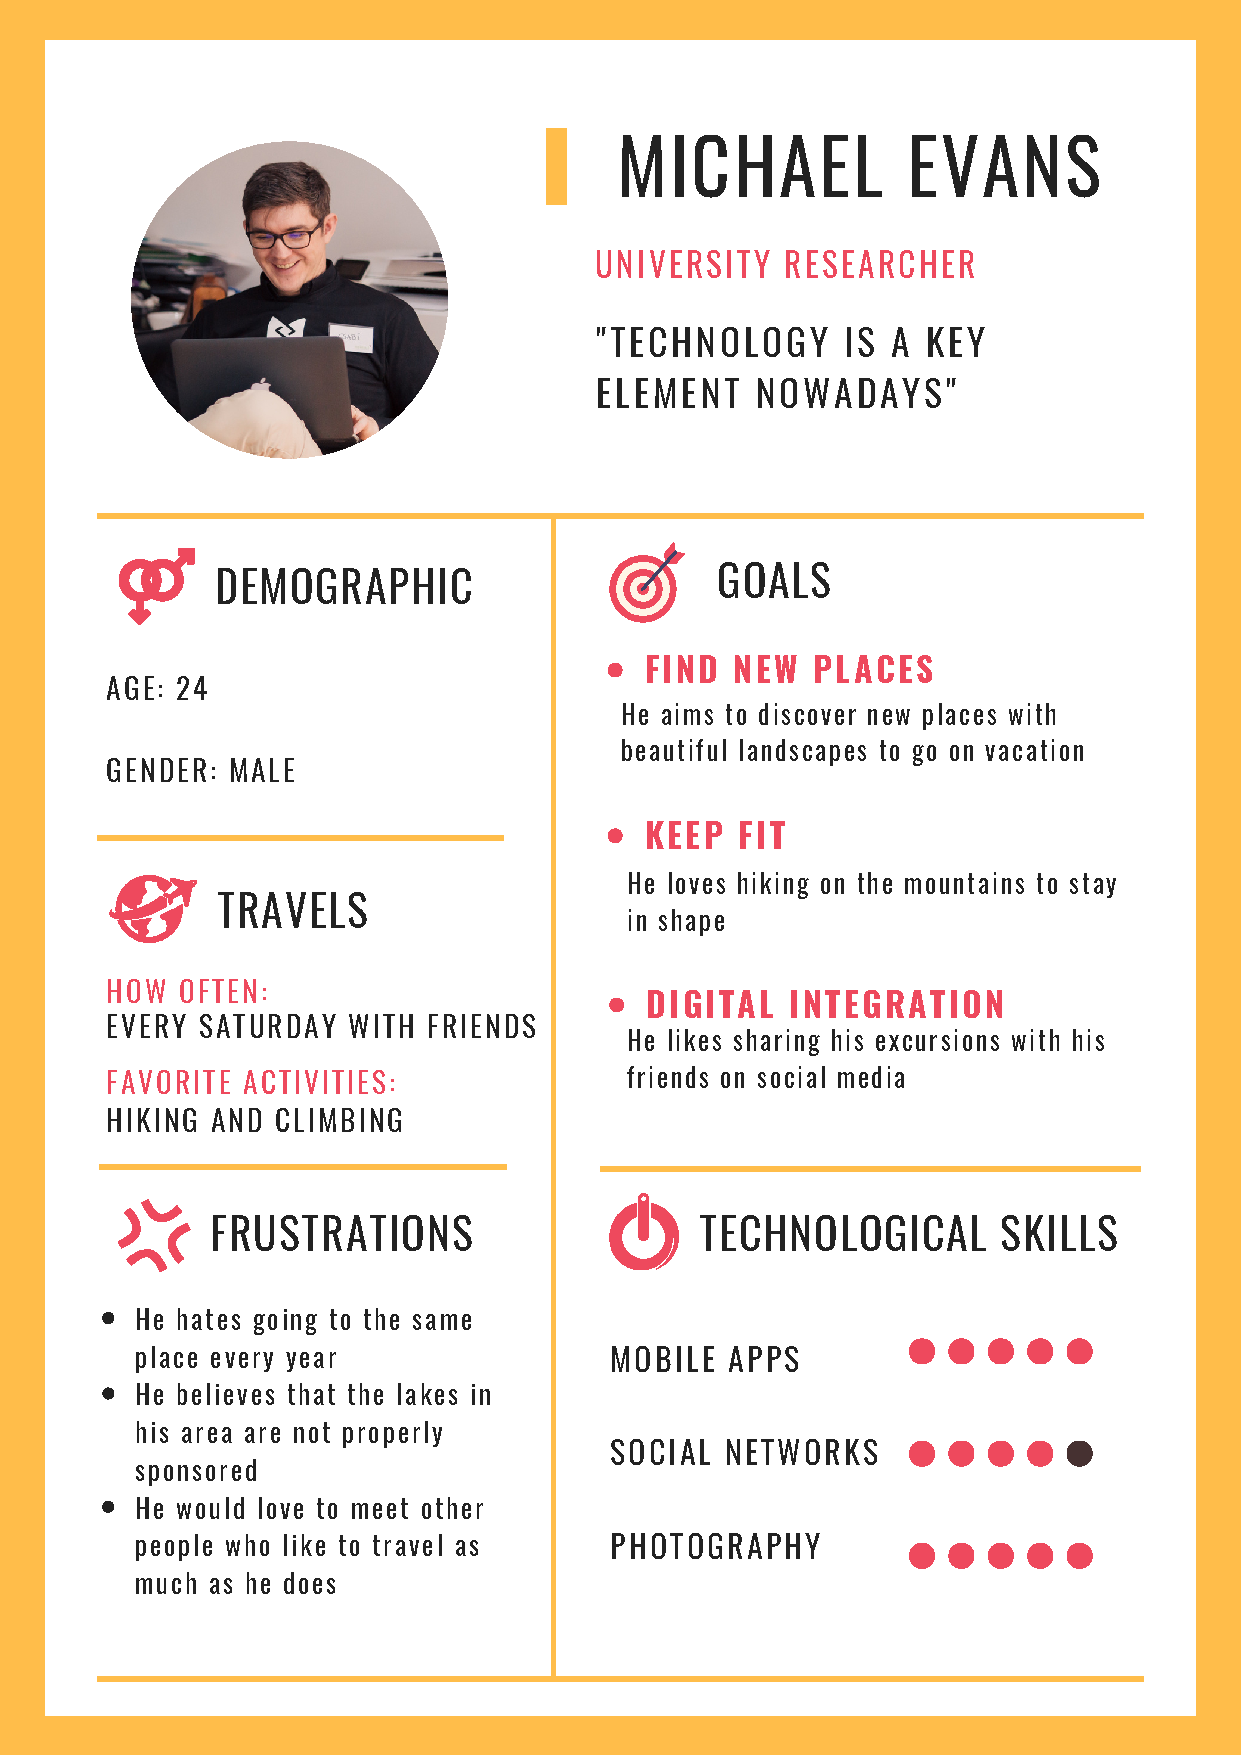
\includegraphics[scale=0.70,page=1]{personas}

\includegraphics[scale=0.70,page=2]{personas}

\section{SWOT}\label{sec:swot}

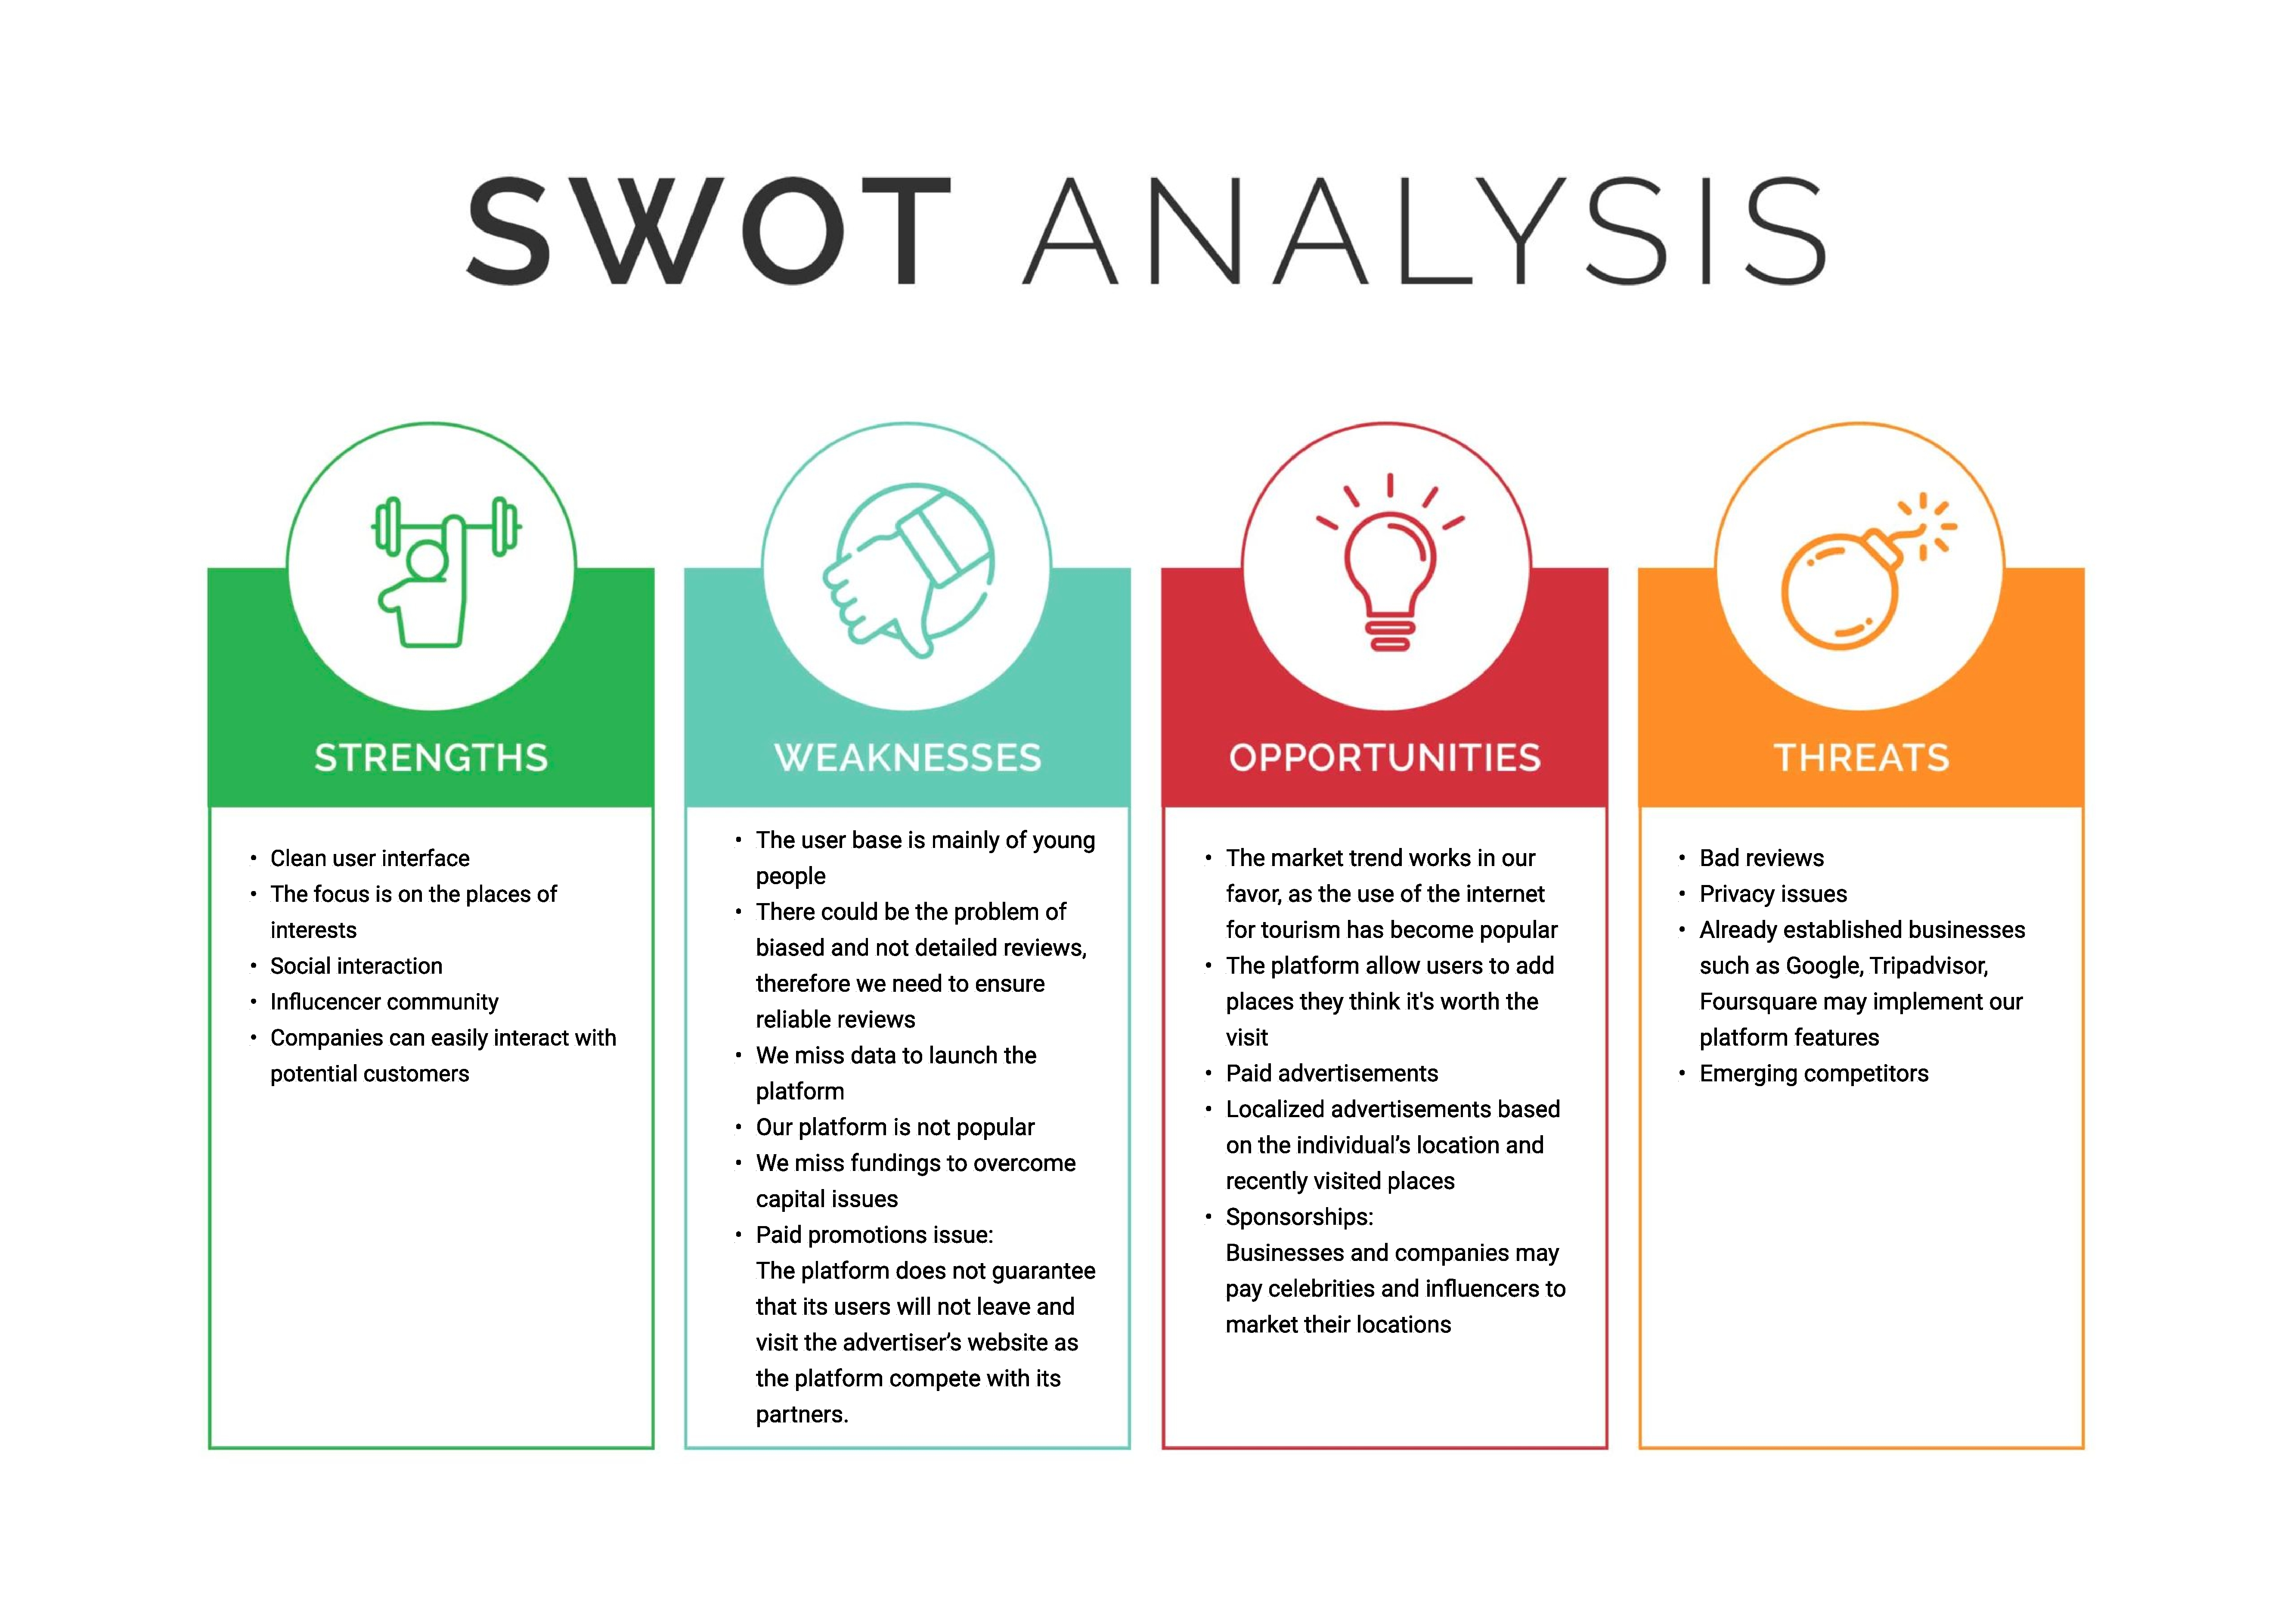
\includegraphics[scale=0.24, angle=90]{swot}

\clearpage

\section{Network effects 2x2 table}\label{sec:network_effects}
\begin{table}[h]
    \newcolumntype{b}{>{\raggedright\arraybackslash}X}
    \newcolumntype{m}{>{\raggedright\arraybackslash\hsize=.8\hsize}X}
    \newcolumntype{s}{>{\hsize=.4\hsize}X}
    \centering
    \begin{tabularx}{\linewidth}{sbm}
         \toprule
            & \textbf{Positive}
            & \textbf{Negative} \\
        \midrule
           \textbf{Same side}
          & The more ordinary users are active on the platform, the more places of interest are present, therefore it is easier for the customers to find the most suitable place for them. 
          
          A greater number of reviews makes the rating of the place more accurate (for the law of large numbers), thus the recommendation system works more effectively. 
          
          The more users are on the application, the more attention it will have, therefore even the possibility of attracting new users will be higher.
          & Due to network congestion, if the number of users grows, the platform needs to be re-scaled, since it should always run as expected.
          
          Since the rise in the number of users inevitably causes a bigger probability to attract people with disruptive behaviours who can harm the community or add non-sense places, we have hired several moderators to admonish such users. \\
          \midrule
          \textbf{Cross side}
          & If the number of ordinary users increases, the possibility for a business user to attract them grows, too. 
          
          On the other hand, the increase in the number of business users necessarily leads to a higher possibility for an ordinary user to find a place of interest.
          &  The more advertisements the platform shows, the less attractive it is to potential customers.\\
        \bottomrule
    \end{tabularx}
    \caption{Four kinds of network effects.}
\end{table}
\end{document}